\documentclass{beamer}

\usepackage[english]{babel}
\usepackage[utf8]{inputenc}
\usepackage{listings}
\usepackage{datetime}
\usepackage{graphics}
\usepackage{fancybox}
\usepackage{color}
\usepackage{courier}
\usepackage[normalem]{ulem}
\usepackage{tikz}
\usetikzlibrary{shapes,arrows,positioning}
\usetheme{CambridgeUS}
\usecolortheme{seagull}
% Changing of bullet foreground color not possible if {itemize item}[ball]
\DefineNamedColor{named}{Purple}{cmyk}{0.52,0.97,0,0.55}
\setbeamertemplate{itemize item}[triangle]
\setbeamercolor{title}{fg=Purple}
\setbeamercolor{frametitle}{fg=Purple}
\setbeamercolor{itemize item}{fg=Purple}
\setbeamercolor{section number projected}{bg=Purple,fg=white}
\setbeamercolor{subsection number projected}{bg=Purple}

\renewcommand{\dateseparator}{.}
\newcommand{\todayiso}{\twodigit\day \dateseparator \twodigit\month \dateseparator \the\year}
\newcommand{\shell}[1]{\texttt{\small #1}}

\title{Osnove korištenja operacijskog sustava Linux}
\subtitle{02. Rad s datotekama i direktorijima}
\author[Antun Aleksa, Josip Žuljević]{Antun Aleksa, Josip Žuljević\\{\small Nositelj: dr. sc. Stjepan Groš}}
\institute[FER]{Sveučilište u Zagrebu \\
				Fakultet elektrotehnike i računarstva}

\date{\todayiso}

\begin{document}
\setbeamertemplate{headline}[]
\setbeamertemplate{footline}{}

\begin{frame}
\maketitle
\end{frame}

\begin{frame}
\frametitle{Sadržaj}
\tableofcontents
\end{frame}

\section{Kopiranje datoteka}
\begin{frame}[t]
\frametitle{Kopiranje datoteka}
\begin{itemize}
  \item Kopiranje se obavlja naredbom \texttt{cp} (engl. \emph{copy})
  \item Sintaksa naredbe
  \begin{itemize}
    \item \texttt{cp \textless datoteka1\textgreater
                     \textless datoteka2\textgreater}
    \begin{itemize}
      \item[-] Stvara kopiju datoteke \texttt{datoteka1} i naziva ju
               \texttt{datoteka2}
    \end{itemize}
    \item \texttt{cp \textless datoteka1\textgreater
                     \textless datoteka2\textgreater
                     \textless direktorij\textgreater}
    \begin{itemize}
      \item[-] Kopira datoteke \texttt{datoteka1} i \texttt{datoteka2} u
               direktorij pod nazivom \texttt{direktorij}
    \end{itemize}
  \end{itemize}
  \item Imena datoteka mogu biti apsolutna ili relativna
\end{itemize}
\end{frame}


%\section{Kopiranje direktorija}
\begin{frame}[t]
\frametitle{Kopiranje direktorija}
\begin{itemize}
  \item Kopiranje direktorija (i svih poddirektorija i datoteka) se
        obavlja zadavanjem opcije \texttt{-r} naredbi \texttt{cp}
  \begin{itemize}
    \item[] \texttt{cp -r \textless direktorij1\textgreater
                          \textless direktorij2\textgreater}
    \item Ako \texttt{direktorij2} ne postoji, bit će kreiran kao kopija
          prvog
    \item Ako \texttt{direktorij2} postoji, \texttt{direktorij1} će biti
          kopiran u njega
  \end{itemize}
  \item Oba argumenta mogu biti apsolutna ili relativna
  \item Dosta naredbi ima neku opciju za rekurziju
\end{itemize}
\end{frame}


\section{Preimenovanje i premještanje datoteka}
\begin{frame}[t]
\frametitle{Preimenovanje i premještanje datoteka}
\begin{itemize}
  \item Premještanje i preimenovanje se obavlja \textbf{jednom} naredbom
        \texttt{mv} \\(engl. \emph{move})
  \item Sintaksa naredbe
  \begin{itemize}
    \item[] \texttt{mv \textless datoteka1\textgreater
                       \textless datoteka2\textgreater}
    \begin{itemize}
      \item Mijenja ime datoteke \texttt{datoteka1} u \texttt{datoteka2}
    \end{itemize}
    \item[] \texttt{mv \textless datoteka1\textgreater
                       \textless datoteka2\textgreater
                       \textless direktorij\textgreater}
    \begin{itemize}
      \item Premješta datoteke \texttt{datoteka1} i \texttt{datoteka2}
               u direktorij pod nazivom \texttt{direktorij}
    \end{itemize}
  \end{itemize}
\end{itemize}
\end{frame}

\begin{frame}[t]
\frametitle{Preimenovanje i premještanje direktorija}
\begin{itemize}
  \item Naredba \texttt{mv} može služiti za preimenovanje direktorija
  \begin{itemize}
    \item Sintaksa je ista kao za premještanje datoteka
    \item Može pomicati i direktorije bez potrebe za dodatnim argumentima
  \end{itemize}
\end{itemize}
\end{frame}

\section{Brisanje datoteka i direktorija}
\begin{frame}[t]
\frametitle{Brisanje datoteka}
\begin{itemize}
  \item Brisanje datoteka i direktorija obavlja se naredbom \texttt{rm}
        (engl. \emph{remove})
  \item Sintaksa naredbe
  \begin{itemize}
    \item[] \texttt{rm \textless ime datoteke\textgreater}
  \end{itemize}
\end{itemize}
\end{frame}

\begin{frame}[t]
\frametitle{Brisanje direktorija}
\begin{itemize}
  \item Za brisanje direktorija koristi se naredba \texttt{rmdir}
  \begin{itemize}
    \item Direktorij mora biti prazan (osim posebnih direktorija)
  \end{itemize}
  \item Sintaksa
  \begin{itemize}
    \item[] \texttt{rmdir \textless ime direktorija\textgreater}
  \end{itemize}
  \item Zadatak
  \begin{itemize}
    \item Pokušati obrisati direktorij \texttt{\$HOME/b}
    \item Pokušati obrisati direktorij \texttt{\$HOME/a}
  \end{itemize}
   \item Ako direktorij nije prazan, možemo koristiti naredbu \texttt{rm}
        sa sljedećim opcijama
  \begin{itemize}
    \item \texttt{-r} rekurzivno brisanje
    \item \texttt{-f} prisilno brisanje
  \end{itemize}
  \item Sintaksa je
  \begin{itemize}
    \item[] \texttt{rm -rf \textless ime direktorija\textgreater\ldots}
  \end{itemize}
  \item[] OPREZNO S TOM NAREDBOM! NEMA POVRATA OBRISANIH PODATAKA!
\end{itemize}
\end{frame}


\section{Nazivi datoteka}
\begin{frame}[t]
\frametitle{Nazivi datoteka (1)}
\begin{itemize}
  \item Linux razlikuje velika i mala slova
  \item Imena datoteka mogu sadržavati sve znakove osim /, koji označava
        poddirektorij
  \item Imena mogu sadržavati praznine
  \begin{itemize}
    \item Praznine obično znače sljedeći argument naredbe
  \end{itemize}
  \item Primjer:
  \begin{itemize}
    \item[] \texttt{\$ mkdir novi direktorij}
    \begin{itemize}
    	\item stvorena dva direktorija \texttt{novi} i \texttt{direktorij}
    \end{itemize}
  \end{itemize}
\end{itemize}
\end{frame}

\begin{frame}[t]
\frametitle{Nazivi datoteka (2)}
\begin{itemize}
  \item Datoteka ili direktorij s prazninama označava se se na dva načina
  \begin{itemize}
  \item Stavljanje imena datoteke pod navodnike (različito značenje jednostrukih i dvostrukih navodnika)
    \item ubacivanje znaka \textbackslash{} (engl. \emph{backslash})
          prije svake praznine
  \end{itemize}
  \item Primjer:
  \begin{itemize}
    \item[] \texttt{\$ mkdir "nova datoteka 2"}
    \item[] \texttt{\$ rmdir nova\textbackslash{} datoteka\textbackslash{}
                     2}
  \end{itemize}
\end{itemize}
\end{frame}

\begin{frame}[t]
\frametitle{Pregled direktorija sustava (1)}
\begin{itemize}
  \item Datotečni sustav na Linuxu je strukturiran kao stablo
  \begin{itemize}
    \item Ima jedan korijenski direktorij ispod kojeg su sve ostale
          datoteke
  \end{itemize}
  \begin{flushleft}
%  \includegraphics[scale=0.5]{filesystem}
  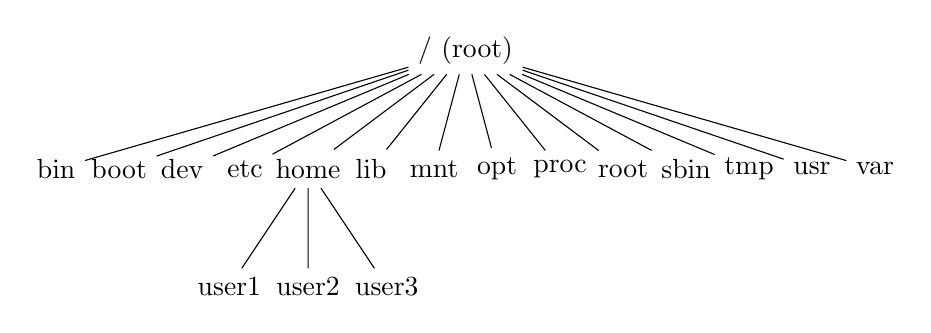
\begin{tikzpicture}[
      level 1/.style={sibling distance=8mm},
      level 2/.style={sibling distance=10mm}
    ]
    \node {/ (root) }
        child {
          node {bin}
        }
        child {
          node {boot}
        }
        child {
          node {dev}
        }
        child {
          node {etc}
        }
        child {
          node {home}
          child {
            node {user1}
          }
          child {
            node {user2}
          }
          child {
            node {user3}
          }
        }
        child {
          node {lib}
        }
        child {
          node {mnt}
        }
        child {
          node {opt}
        }
        child {
          node {proc}
        }
        child {
          node {root}
        }
        child {
          node {sbin}
        }
        child {
          node {tmp}
        }
        child {
          node {usr}
        }
        child {
          node {var}
        }
      ;
  \end{tikzpicture}
\end{flushleft}


\end{itemize}
\end{frame}

\begin{frame}[t]
\frametitle{Pregled direktorija sustava (2)}
\begin{itemize}
  \item Sadržaj datoteka definiran je FHS standardom\\ (engl.
        \emph{Filesystem Hierarchy Standard})
  \begin{itemize}
    \item Struktura sustava ipak nije ista za sve Unix sustave
  \end{itemize}
  \item Definirani su direktoriji neposredno ispod korijenskog direktorija
        i neki njihovi poddirektoriji
  \item[] \texttt{/}
  \begin{itemize}
    \item Datotečni sustav organiziran je u hijerarhiju koja počinje od
          \texttt{/} (\emph{root})
  \end{itemize}
\end{itemize}
\end{frame}

\begin{frame}[t]
\frametitle{Pregled direktorija sustava (3)}
\begin{itemize}
  \item[] \texttt{/bin}
  \begin{itemize}
    \item Korisnički i administratorski alati bez obzira da li je sustav u
          jednokorisničkom ili višekorisničkom načinu rada
  \end{itemize}
  \item[] \texttt{/boot}
  \begin{itemize}
    \item Jezgra operacijskog sustava i sve potrebno kako bi se operacijski
          sustav mogao pokrenuti tijekom podizanja sustava
          (engl. \emph{booting})
  \end{itemize}
\end{itemize}
\end{frame}

\begin{frame}[t]
\frametitle{Pregled direktorija sustava (4)}
\begin{itemize}
  \item \texttt{/dev}
  \begin{itemize}
    \item Direktorij s posebnim datotekama koje predstavljaju različite
          uređaje
  \end{itemize}
  \item \texttt{/etc}
  \begin{itemize}
    \item Konfiguracijske datoteke cijelog sustava
  \end{itemize}
  \item \texttt{/lib} (\texttt{/lib64})
  \begin{itemize}
    \item Biblioteke nužne za rad sustava
    \item Tu se nalaze moduli operacijskog sustava.
  \end{itemize}
\end{itemize}
\end{frame}

\begin{frame}[t]
\frametitle{Pregled direktorija sustava (5)}
\begin{itemize}
  \item \texttt{/lost+found}
  \begin{itemize}
    \item Datoteke vračene nakon pada sustava
  \end{itemize}
  \item \texttt{/media}
  \begin{itemize}
    \item Direktorij unutar kojega se automatski dodaju pokretni
          uređaji/mediji kada se priključe na računalo, primjerice
          CD-ROM-ovi, USB diskovi, \ldots
  \end{itemize}
  \item \texttt{/mnt}
  \begin{itemize}
    \item Direktorij na koji (ili unutar kojega) korisnik ručno dodaje
          pokretne uređaje/medije
  \end{itemize}
\end{itemize}
\end{frame}

\begin{frame}[t]
\frametitle{Pregled direktorija sustava (6)}
\begin{itemize}
  \item \texttt{/opt}
  \begin{itemize}
    \item Instalacije programa koji nisu dio standardnog sustava
    \item Programi i pripadajuće datoteke se nalaze unutar jednog
          direktorija.
  \end{itemize}
  \item \texttt{/proc}
  \begin{itemize}
    \item Sadrži virtualne datoteke koje se mijenjaju ovisno o stanju
          sustava
    \item Pisanje u neku od datoteka može promijeniti ponašanje sustava.
  \end{itemize}
\end{itemize}
\end{frame}


\begin{frame}[t]
\frametitle{Pregled direktorija sustava (7)}
\begin{itemize}
  \item \texttt{/sbin}
  \begin{itemize}
    \item Sistemski programi koje administrator sustava treba imati na
          raspolaganju za podizanje sustava.
  \end{itemize}
  \item \texttt{/tmp}
  \begin{itemize}
    \item Direktorij za privremenu pohranu datoteka
    \item U njega mogu pisati svi korisnici i najčešće ga koriste
          aplikacije za spremanje datoteka tijekom rada
  \end{itemize}
\end{itemize}
\end{frame}

\begin{frame}[t]
\frametitle{Pregled direktorija sustava (8)}
\begin{itemize}
  \item \texttt{/var}
  \begin{itemize}
    \item Datoteke koje se često mijenjaju poput logova i pošte
  \end{itemize}
  \item \texttt{/srv}
  \begin{itemize}
    \item Direktoriji s podacima koji se nude korisnicima preko servisa
    \item Primjer su web stranice preko HTTP protokola i binarne datoteke
          preko FTP protokola.
  \end{itemize}
\end{itemize}
\end{frame}

\begin{frame}[t]
\frametitle{Pregled direktorija sustava (9)}
\begin{itemize}
  \item \texttt{/home}
  \begin{itemize}
    \item Matični direktoriji korisnika smješteni su unutar ovog
          direktorija
    \item Svaki korisnik posjeduje svoj direktorij gdje se nalaze osobne
          datoteke korisnika
    \item Postavke aplikacija za pojedinog korisnika nalaze se u njegovom
          matičnom direktoriju, u skrivenim datotekama.
  \end{itemize}
  \item \texttt{/root}
  \begin{itemize}
    \item Matični direktorij \emph{root} korisnika
  \end{itemize}
\end{itemize}
\end{frame}

\section{Struktura \texttt{usr} direktorija}
\begin{frame}[t]
\frametitle{Struktura \texttt{usr} direktorija (1)}
\begin{itemize}
  \item \texttt{/usr}
  \begin{itemize}
    \item Sadrži vlastitu strukturu
    \item Za razliku od \texttt{/sbin} i \texttt{/bin} direktorija, koji
          sadržavaju programe za osnovnu funkcionalnost sustava, ovdje su
          programi za normalan rad sa sustavom
    \item[]
    \item[] \texttt{/usr/bin}
    \begin{itemize}
      \item Korisnički programi za opći rad sa sustavom
    \end{itemize}
    \item[] \texttt{/usr/sbin}
    \begin{itemize}
      \item Programi za cjelokupnu administraciju sustava
    \end{itemize}
  \end{itemize}
\end{itemize}
\end{frame}

\begin{frame}[t]
\frametitle{Struktura \texttt{usr} direktorija (2)}
\begin{itemize}
  \item Raspodjela \texttt{/usr},\texttt{/bin} i \texttt{/sbin} nije uvijek
        precizno definirana i ovisi o implementaciji Unix sustava
  \item[]
  \item[] \texttt{/usr/local}
  \begin{itemize}
    \item Instalacije programa na lokalnom sustavu
    \item Sadrži poddirektorije \texttt{/usr/local/bin} i
          \texttt{/usr/local/sbin}
    \item U \texttt{/usr/local} nalazili su se programi specifični za
          pojedinog korisnika, dok su se u ostalim direktorijima nalazili
          programi za sve korisnike
  \end{itemize}
\end{itemize}
\end{frame}

\section{Pregled zauzeća diskovnog prostora}
\begin{frame}[t]
\frametitle{Naredba \texttt{df}}
\begin{itemize}
  \item Naredba \texttt{df} ispisuje zauzeće po particijama
  \begin{itemize}
    \item Najčešće se koristi s opcijom \texttt{-h}
  \end{itemize}
  \item Zauzeće prostora po direktorijima se provjerava naredbom
        \texttt{du}
  \item Moguće je ispisivanje zauzeća po poddirektorijima do određene
        razine
\end{itemize}
\end{frame}

\section{Unix datoteke}
\begin{frame}[t]
\frametitle{Unix datoteke (1)}
\begin{itemize}
  \item Na Unix sustavima je sve datoteka
  \item Posebne vrste datoteka postoje zbog različitih pristupa dijelova
        sustava
  \begin{itemize}
    \item Tipkovnice
    \item Diskovi
    \item Zvučne kartice
    \item \ldots
  \end{itemize}
\end{itemize}
\end{frame}

\begin{frame}[t]
\frametitle{Unix datoteke (2)}
\begin{itemize}
  \item Vrsta datoteke određuje se naredbom \shell{ls}
  \item Prvi znak pri dugom ispisu određuje tip datoteke
  \item Primjer
  \begin{itemize}
    \item Stvoriti direktorij i ispisati informacije o njemu
  \end{itemize}
  \item[] \shell{\$ mkdir direktorij}
  \item[] \shell{\$ ls -ld direktorij}
  \item[] \shell{\footnotesize\textbf{d}rwxr-xr-x 2 cetko cetko 4096
                          2010-10-28 12:39 direktorij/}
\end{itemize}
\end{frame}

\begin{frame}[t]
\frametitle{Obična datoteka}
\begin{itemize}
  \item Standardna datoteka, prva asocijacija na riječ datoteka
  \item Prazna datoteka stvara se naredbom \shell{touch} bez argumenata
\end{itemize}
\end{frame}


\begin{frame}[t]
\frametitle{Imenovani cjevovod}
\begin{itemize}
  \item engl. \emph{named pipe}
  \item Cjevovodi služe za povezivanje izlaza i ulaza dva procesa (engl.
        \emph{interprocess communication})
  \begin{itemize}
    \item Obični cjevovodi postoje samo dok traje komunikacija
    \item Imenovani cjevovodi postoje kao datoteke na sustavu za
          komunikaciju procesa po potrebi
  \end{itemize}
  \item Označava se znakom \textbf{p}
  \item Više o cjevovodima kasnije
\end{itemize}
\end{frame}

\begin{frame}[t]
\frametitle{Direktorij}
\begin{itemize}
  \item Uz svaki direktorij vezana je lista s pripadajućim datotekama
  \item Okosnica strukture sustava
  \item Direktorij obilježava znak \textbf{d} kod ispisa naredbom
        \shell{ls -ld}
\end{itemize}
\end{frame}

\begin{frame}[t]
\frametitle{Priključnica}
\begin{itemize}
  \item engl. \emph{socket}
  \item Služi za komununikaciju procesa preko mreže
  \begin{itemize}
    \item Privremene datoteke
  \end{itemize}
  \item Označava se znakom \textbf{s}
  \item O priključnicama neće biti daljnjih tema
\end{itemize}
\end{frame}

\section{Datoteke uređaja}
\begin{frame}[t]
\frametitle{Datoteke uređaja (1)}
\begin{itemize}
  \item Datoteke uređaja (engl. \emph{device files}) služe za komunikaciju
        s vanjskim uređajima
  \begin{itemize}
    \item Nalaze se u \shell{/dev} direktoriju
  \end{itemize}
  \item Uređaji komuniciraju sa sustavom u blokovima ili znak po znak
\end{itemize}
\end{frame}

\begin{frame}[t]
\frametitle{Datoteke uređaja (2)}
\begin{itemize}
  \item Blok datoteke
  \begin{itemize}
    \item Prijenos podataka odvija se u blokovima
    \item Diskovi, CD-ROM uređaji i memorije
  \end{itemize}
  \item Označavaju se znakom \textbf{b}
  \item Znakovne (engl. \emph{char}) datoteke
  \begin{itemize}
    \item Prijenos podataka znak po znak
    \item Tipkovnice i zvučne kartice
  \end{itemize}
  \item Označavaju se znakom \textbf{c}
\end{itemize}
\end{frame}

\section{Simboličke poveznice}
\begin{frame}[t]
\frametitle{Simboličke poveznice (1)}
\begin{itemize}
  \item engl. \emph{symbolic link}
  \item Poveznice služe za brže pristupanje podacima
  \begin{itemize}
    \item Poput prečaca (engl. \emph{shortcut}) na Windows sustavu
  \end{itemize}
  \item Naredbom \shell{ln -s} stvaraju se simboličke poveznice
\end{itemize}
\end{frame}

\begin{frame}[t]
\frametitle{Simboličke poveznice (2)}
\begin{itemize}
  \item Primjer:
  \begin{itemize}
    \item[] \shell{\$ ln -s a b}
    \item[] \shell{\$ ls -l b}
    \item[] \shell{\footnotesize lrwxrwxrwx 1 cetko cetko 1 2010-10-28 19:18 b -> a}
  \end{itemize}
  \item Poveznice mogu referencirati apsolutne i relativne putanje
  \item Brisanjem simboličke poveznice podaci ostaju na sustavu
\end{itemize}
\end{frame}


\begin{frame}[t]
\frametitle{Pregled sadržaja datoteke}
\begin{itemize}
  \item Ako želimo vidjeti sadržaj neke datoteke na zaslonu možemo
        upotrijebiti naredbu \shell{cat}
  \begin{itemize}
    \item Sintaksa naredbe je
    \item[] \shell{cat \textless ime datoteke\textgreater}
  \end{itemize}
\end{itemize}
\end{frame}

\section{MAC vremena}
\begin{frame}[t]
\frametitle{MAC vremena (1)}
\begin{itemize}
  \item Svaka datoteka/direktorij ima definirana tri vremena
  \begin{itemize}
    \item Vrijeme zadnje promjene (\emph{mtime})
    \begin{itemize}
      \item Naredba \shell{ls} ispisuje ovo vrijeme ako se drugačije
               ne kaže!
    \end{itemize}
    \item Vrijeme zadnjeg pristupa (\emph{atime})
    \begin{itemize}
      \item Naredba \shell{ls} će ispisati ovo vrijeme opcijom
            \shell{-u}
    \end{itemize}
    \item Vrijeme zadnje promjene metainformacije (\emph{ctime})
    \begin{itemize}
      \item Ovo vrijeme se ispisuje opcijom \shell{-c}
    \end{itemize}
  \end{itemize}
\end{itemize}
\end{frame}

\begin{frame}[t]
\frametitle{MAC vremena (2)}
\begin{itemize}
  \item Detaljne informacije o datotekama ispisuje naredba \shell{stat},
        uključujući i MAC vremena
  \item Naredba \shell{touch} sva vremena postavlja na trenutno
\end{itemize}
\end{frame}

\begin{frame}[t]
\frametitle{Naredba \shell{file} (1)}
\begin{itemize}
  \item Ponekad imamo na raspolaganju datoteku za koju ne znamo kakvog je
        tipa
  \item U tom slučaju na raspolaganju nam je naredba \shell{file}
  \begin{itemize}
    \item Ona pokušava odrediti vrstu datoteke na osnovu baze tipova
          datoteka
  \end{itemize}
  \item Sintaksa je:
  \begin{itemize}
    \item[] \shell{file <ime datoteke>}
    \end{itemize}
\end{itemize}
\end{frame}

\begin{frame}[t]
\frametitle{Naredba \shell{file} (2)}
\begin{itemize}
  \item Prilično kompleksna naredba koja ne daje točne rezultate u 100\%
        slučajeva, ali je ipak izuzetno korisna
  \item Napomena: tip datoteke u ovom slučaju se razlikuje od definicije
        Unix datoteka
  \begin{itemize}
    \item Pomoću tipa datoteke određuje se koja aplikacija je zadužena za
          pristupanje datoteci
  \end{itemize}
  \item Unix/Linux ne prepoznaje tipove po ekstenzijama
  \begin{itemize}
    \item Svaka ``ekstenzija'' je samo dio imena datoteke
  \end{itemize}
\end{itemize}
\end{frame}

\section{Pregled sadržaja datoteke}
\begin{frame}[t]
\frametitle{Pregled dijela sadržaja datoteke (1)}
\begin{itemize}
  \item Ako je datoteka prevelika nećemo ništa vidjeti
  \begin{itemize}
    \item Primjer datoteke \shell{/usr/include/stdio.h}
    \item Ako je datoteka prevelika, a zanima nas samo prvih N redaka,
          možemo upotrijebiti naredbu \shell{head}
  \end{itemize}
  \item Sintaksa datoteke je:
  \begin{itemize}
    \item[] \shell{head [-n <n>] <ime datoteke>}
    \item Ako se ne navede opcija, ispisuje prvih 10 redaka, inače ispisuje prvih N redaka
  \end{itemize}
  \item Ako je \shell{<n>} negativan, ispisuje sve osim zadnjih n redaka
\end{itemize}
\end{frame}

\begin{frame}[t]
\frametitle{Pregled dijela sadržaja datoteke (2)}
\begin{itemize}
  \item Ako nas zanima samo zadnjih N redaka,možemo upotrijebiti
        naredbu \shell{tail}
  \begin{itemize}
    \item Sintaksa datoteke je:
    \item[] \shell{tail [-n <n>] <ime datoteke>}
  \end{itemize}
  \item Ako se ne navede opcija, ispisuje zadnjih 10 redaka, inače ispisuje
        zadnjih N redaka
  \item Ako je \shell{<n>} pozitivan (ima znak +) ispisuje od zadanog
        retka do kraja!
\end{itemize}
\end{frame}

\begin{frame}[t]
\frametitle{Pregledavanje datoteka po stranicama (1)}
\begin{itemize}
  \item Ako želimo pregledavati sadržaj datoteke stranicu po stranicu, na
        raspolaganju imamo naredbe \shell{less} ili \shell{more}
  \item ``Stranica'' je količina teksta koja stane na jedan ekran!
  \begin{itemize}
    \item \shell{less} je novija varijanta sa većim mogućnostima
  \end{itemize}
  \item Standard na Linuxu, ali nije dostupna na komercijalnim Unix
        sustavima
  \item Obje naredbe kao argument primaju ime datoteke
  \begin{itemize}
    \item Izlazak iz pregledavanja je s tipkom q
    \item Naredba \shell{man} koristi te programe za prikaz uputa!
  \end{itemize}
\end{itemize}
\end{frame}

\section{Mijenjanje sadržaja datoteka}
\begin{frame}[t]
\frametitle{Mijenjanje sadržaja datoteka}
\begin{itemize}
  \item Postoji nekoliko tekstualnih editora na Linuxu
  \item Često korišteni su \shell{nano} i \shell{vim}
  \item Editori \shell{nano} i \shell{vi} su dio standardne instalacije većine Linux distribucija
\end{itemize}
\end{frame}

\section{Pregled naredbi}
\begin{frame}[t]
\frametitle{Pregled naredbi}
\begin{tabular}{| l | c |} \hline
  \shell{cp} & kopiranje datoteka/direktorija \\ \hline
  \shell{mv} & preimenovanje i premještanje datoteka/direktorija \\ \hline
  \shell{rm} & brisanje datoteka/direktorija \\ \hline
  \shell{rmdir} & brisanje direktorija \\ \hline
  \shell{df} & ispis zauzeća po particijama \\ \hline
  \shell{du} & zauzeće prostora po direktorijima \\ \hline
  \shell{touch} & stvaranje prazne datoteke \\ \hline
  \shell{ln -s} & stvaranje simboličke poveznice \\ \hline
  \shell{cat} & pregled sadržaja datoteke \\ \hline
  \shell{stat} & detaljnje informacije o datoteci/direktoriju \\ \hline
  \shell{file} & ispis tipa datoteke \\ \hline
  \shell{head} & ispis prvih 10 redaka datoteke (\shell{[-n <n>]} = prvih n redaka) \\ \hline
  \shell{tail} & ispis zadnjih 10 redaka datoteke (\shell{[-n <n>]} = zadnjih n redaka) \\ \hline


\end{tabular}
\end{frame}

\end{document}
